\documentclass[11pt]{article}
\usepackage{geometry}                % See geometry.pdf to learn the layout options. There are lots.
\geometry{a4paper}                   % ... or a4paper or a5paper or ... 
%\geometry{landscape}                % Activate for for rotated page geometry
%\usepackage[parfill]{parskip}    % Activate to begin paragraphs with an empty line rather than an indent
\usepackage{graphicx}
\usepackage{amssymb}
\usepackage{epstopdf}
\usepackage[german, english]{babel}
\usepackage[utf8]{inputenc}
\usepackage{hyperref}
\usepackage{multicol}
\usepackage[table]{xcolor}% http://ctan.org/pkg/xcolor

\DeclareGraphicsRule{.tif}{png}{.png}{`convert #1 `dirname #1`/`basename #1 .tif`.png}

%\date{}                                           % Activate to display a given date or no date

\hyphenation{Le-on-ding}

\begin{document}
\begin{titlepage}
\begin{flushright}

\includegraphics[scale=.10]{img/DRAFT-RoboDucks-Logo.jpg}\\
\end{flushright}

\vspace{2em}

\begin{center}
{\Huge Humanoid Robotics @ HTL Leonding} \\[2em]
\includegraphics[scale=0.55]{img/Titlepage.png}\\[2em]
{\LARGE Annual Report 2019 / 2020}
\end{center}
\end{titlepage}

\tableofcontents
\newpage

\section{Introduction}
This report lists the activities of the Humanoid Robotics Team at the HTL Leonding during the school year~2019/2020, i.e., from September 1, 2019 to August 31, 2020. The Humanoid Robotics Team may look back to a rather mixed year. On the one hand we were pretty successful to even increase our team size, made a big step in our soccer software towards a competitive version, and had a number of great events with a high public resonance. On the other hand the COVID-19 pandemic also hit us and we were not able to take part in the RoboCup Challenges since they were quit altogether this year.

In order to keep the report short a good amount of details is missing here. More details could be found on \url{http://roboducks.htl-leonding.ac.at}. If there are any further questions the team lead can be contacted via \\[1em]
Peter Bauer\\
HTL Leonding, Department of Informatics\\
Limesstraße 12 -- 14\\
4060 Leonding\\
Fon: +43 676 6173320\\
Mail: p.bauer@htl-leonding.ac.at

\section{About Humanoid Robotics @ HTL Leonding}\label{sec:about}
Humanoid Robotics @ HTL Leonding is an initiative to motivate students of the HTL Leonding to deal with autonomous systems in general and with humanoid robots in particular. Furthermore students shall gain first experience in working on a software project within a larger team which implies the usual parameters like communication issues between team members, significantly large code bases, need for documentation, thorough tests, etc. Finally strictly motivate our students to take part in different robot competitions offered by the RoboCup Organization to get a clear feedback how well our teams are doing their job.

Since the HTL Leonding has a clear focus on software and no expertise in mechanical engineering a robot platform called {\em Nao} which is a standard platform from Softbank Robotics is used. This platform includes a humanoid robot (as it can be seen on the title page), an operating system called NAOqi which is a Linux kernel augmented by a set of libraries to control the robot's hardware and a set of software tools to program the robot. The Naos can be programmed in a great number of different programming languages but a proprietary graphical environment (Choregraphe), Python, and  C++ is mainly used.

As it requires already a good knowledge in software development and its related tooling to handle the C++ development stack we do an introductory phase for second graders where Choregraphe can be used as a programming environment.

After this the students may chose to move into the so-called soccer team which prepares to take part in the Standard Platform League which is a soccer competition where only Naos are allowed to take part. Here the Naos have to act autonomously as soccer players where two teams of five Naos play a soccer game on a 9 x 6 m large field. To program the robots it is necessary to work deeply in the fields of computer vision, strategy, planning, motion, etc. Therefore, only university level schools take part in this league and it is one of the big goals to take part as the first technical college being formally on pre-university level.

\section{Environmental Changes from Last Year}
As described in section~\ref{sec:about} the young students newly joining our team are requested to accomplish smaller programming tasks by using the Softbank Robotics proprietary Choregraphe. In the past years the students had to take part in the {\em Demo Humanoid Challenge} of the RoboCup Junior Austrian Open where less complex programming tasks which can be mastered by freshmen are requested.

Unfortunately the RoboCupJunior Austrian Open decided to discontinue the Demo Humanoid Challenge and our junior team members were not able to proof themselves in this great competition. At this point we are busy to find a competition which can provide a similarly motivating spirit as the Demo Humanoid Challenge.

Furthermore the COVID-19 pandemic destroyed our plans to take part in the RoboCup German Open in April. As of today the organizing committee of the RoboCup German Open schedules a competition from April 21 to 24 in Magdeburg. We will try hard to attend this competition.

\section{The Team}
Building a strong team of students and teachers who do a very focused work is an all time target we have in mind. Especially a smooth hand-over from one student generation to a next is a central topic. The more we are happy that we were able to increase the head count from eighteen  to 23 developers compared to the last period under report. The team members are the following: 

\begin{multicols}{2}
\begin{itemize}
	\item Erik Mayrhofer (5BHIF)
	\item Jan Neuburger (5BHIF)
	\item Florian Schwarcz (5BHIF)
	\item Max Wal (5BHIF)
	\item Matthias Bal (3AHIF)
	\item Emina Sljivic (3AHIF)
	\item Robert Freiseisen (3BHIF)
	\item Simon Holzapfel (3BHIF)
	\item Marc Kruiß (3BHIF)
	\item Quirin Ecker (3AHITM)
	\item Philipp Edlinger (3AHITM)
	\item Vanessa Primetzhofer (3AHITM)
	\item Theresa Holzer (2AHITM)
	\item Lara Pichler (2AHITM)
	\item Sarah Reichl (2AHITM)
	\item David Wögerbauer (2AHITM)
	\item Jakob Rathberger (2AHIF)
	\item Imad Crnčević (2BHIF)
	\item Alessandro Detta (2BHIF)
	\item Nikos Hagenberger (2BHIF)
	\item Berkan Kücüklü (2BHIF)
	\item Moritz Preining (2BHIF)
	\item Clemens Wolfmayr (2BHIF)
\end{itemize}
\end{multicols}

\noindent Since our promotional activities in terms of generating new artifacts could be reduced during this period under report it was not necessary to have a separate promotion team.

Compared to the last annual report 2019 we can still see a positive development in terms of our head count. Nevertheless we have to keep in mind that four of our students attended the $5^{\textrm{\small th}}$ grade and drop out by end of this period. So we will again try to motivate a high number of talented and motivated $2^{\textrm{\small nd}}$ graders to join our team this fall. Since the team of mentors was involved in the programming courses of the first graders this year we had already the chance to see the programming skills of the students in these classes and already startet to motivate the best of them to join our team next year.

The split of our team into an experienced and a freshman sub team which we introduced in 2017 proved to work well. Therefore we continued this practice. The team of the experienced students is still  working on a software for the Nao Standard Platform League. The freshman team was busy to implement a number of introductory examples which were used during our demo and training events in different schools (see~\ref{sec:activities_overview}).

Finally it is worth mentioning that we succeeded to get another mentor into our Team: Dietmar Steiner. He joined the HTL Leodning two years ago and will take over parts of our soccer team management. With him we have now three mentors and can guarantee a good support for our students in technical as well as organizational matters.

\begin{figure}[b]
\begin{center}

\includegraphics[scale=0.38]{img/fabasoft.png}
\hfill

\includegraphics[scale=0.38]{img/absleoLogo.png}
\end{center}
%\caption*{}
\end{figure}

\section{RoboDojo – Partnership with Fabasoft}
Based on the experience we have made from 2017 onwards where we organized extra development sprints together with and at {\em Fabasoft} we tried to get the schedule of theses sprints more predictable. Therefore we organized a regular jour fixe every second Friday from 3 to 7 pm. Additionally we organized meetings during school holidays when students were not blocked because of regular school courses. Again we were lucky to partner with Fabasoft which kindly provided a great working environment and a catering for these extra sprints. In order to prepare for a broader communication of these sprints we decided to summarize these activities under the name of {\em RoboDojo}. As in the last years the RoboDojo was greatly accepted by the students and we had productive days.

The sponsoring contract between Fabasoft and the Humanoid Robotics @ HTL Leonding was continued and we were able to increase our Nao fleet by four more robots. We tried to pay this back with a number of public events (see section~\ref{sec:activities_overview}).

\section{Activities}\label{sec:activities_overview}
In this period under report we had a number of eleven public appearances at eight different events. Besides these we continued our efforts to write a software for the Standard Platform League of the RoboCup and to get web site of Humanoid Robotics @ HTL Leonding.

The following list gives a brief overview of the events during the last period. A more detailed description of the events can be found under \url{http://roboducks.htl-leonding.ac.at/posts/2019_20/}.

\begin{figure}
\begin{center}
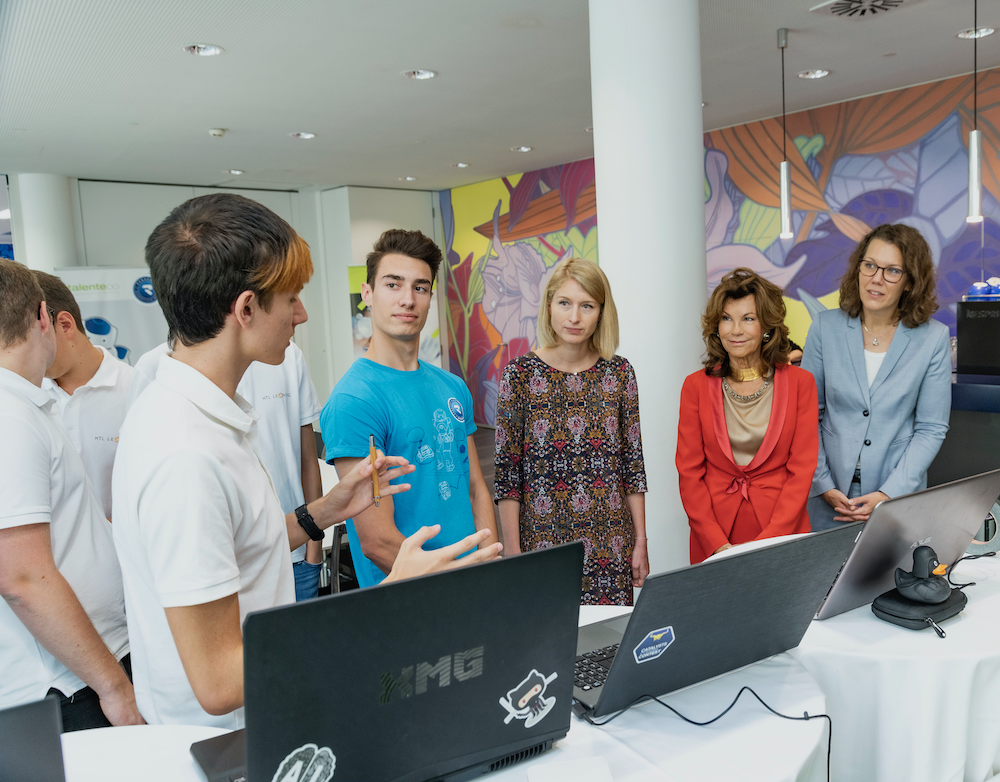
\includegraphics[scale=0.25]{img/activityImage1.png}
\end{center}
\caption{Visit of Chancellor Bierlein, Fed. Minister Rauskala, and Dpt. Gov. Haberlander}
\label{fig:ballDerLeondinger}
\end{figure}

\begin{figure}
\begin{center}
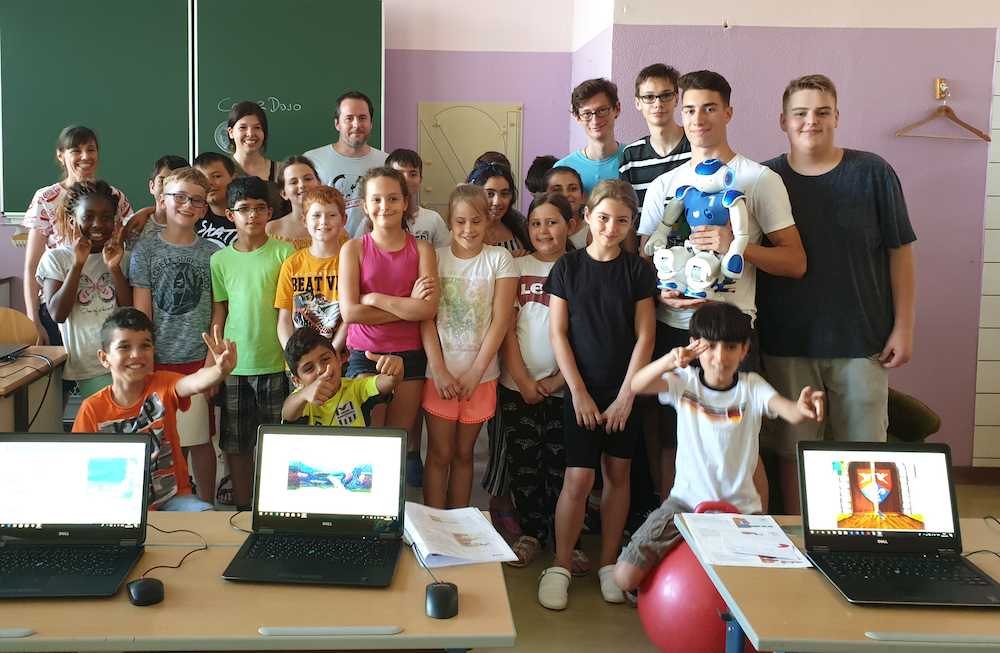
\includegraphics[scale=0.25]{img/activityImage2.png}
\end{center}
\caption{RoboDojo at NMS Lambach}
\label{fig:rcjWinners}
\end{figure}

\begin{itemize}
	\item September 5, 2019: Visit of chancellor Brigitte Bierlein, Federal Minister Iris Rauskala and Deputy Governor Christine Haberlander
	\item October 2 to 4, 2019: Messe Jugend und Beruf, Wels
	\item  October 10, 2019: Hofer KG ALPHA TALK, Eberstalzell
	\item  October 11, 2019: Coder Dojo Special Event @ HTL Leonding
	\item  December 12, 2019: Summit Indurstrie 4.0, Linz
	\item  December 19, 2019: CoderDojo at the NMS 2, Lambach
	\item  January 10, 2020: My Informatics World CoderDojo, Leonding
	\item  January 23, 2020: Open Doors Day, HTL Leonding
\end{itemize}

\begin{figure}
\begin{center}
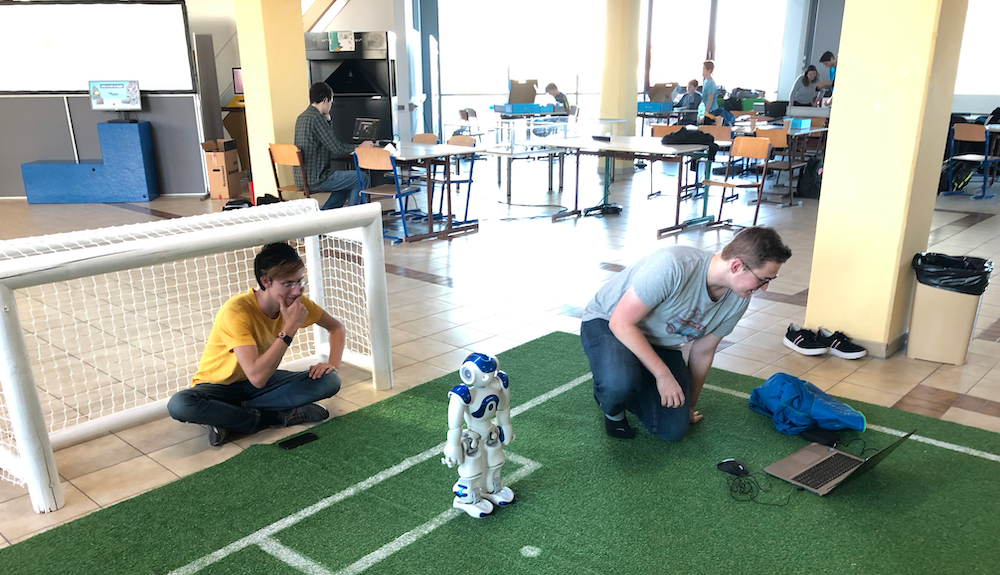
\includegraphics[scale=0.25]{img/activityImage3.png}
\end{center}
\caption{RoboDojo at HTL Leonding}
\label{fig:soccerTraining}
\end{figure}

\section{Finance}
\subsection{Target-Performance Evaluation 2019/20}\label{sec:tpe}
Overall we spent € 12,758.96 during the last period. Compared to our budget we spent € 2,641.04 less than expected. This is due to the fact that SoftBank Robotics was not able to bill us the maintenance contracts for two Naos (Tom and Anastasia). Since we expect SoftBank Robotics to get this fixed by start of next school year we transfer this money into our next period. Details of the TPE can be found in figure~\ref{fig:tpe}.
\begin{figure}
\begin{center}
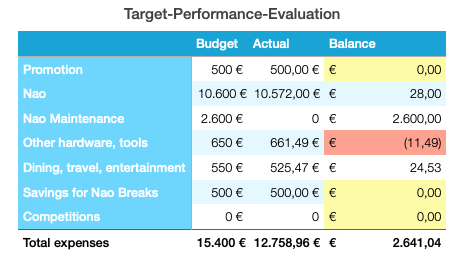
\includegraphics[scale=0.5]{img/targetPerformanceEvaluation.png}
\end{center}
\caption{Target-Performance Evaluation for 2019/20}
\label{fig:tpe}
\end{figure}

\subsection{Budget 2020/21}\label{sec:budget}
For the upcoming period we expect a total income of € 31,220. The main part is estimated to come from our sponsoring contract with Fabasoft. Furthermore we asked the HTL Leonding to support the main portion of the maintenance costs for our Naos. A new position on our income side will be some fees for public demonstrations of our soccer team. In particular we sent a quote to the organizing committee of the RoboCupJunior Austrian Open 2021 in Weiz.

The expenses side of our budget is dominated by financing the participation at the RoboCup German Open in Magdeburg. We plan to go there with a number of 15 students. This is necessary since the handling of the Nao soccer team under competition conditions needs about 8 students. Furthermore a number of about 5 students will document our games from the side lines. The team will be completed by two to three mentors.

The second and third largest points are the Nao maintenance and the purchase of a new Nao. As already mentioned in section~\ref{sec:tpe} we expect to be charged for a two years maintenance for Anastasia and Tom. Additionally we have to start the maintenance for Margret and Donald since their default maintenance contracts end by October 2020. Since the Naos V6 have a much better performance than the V5 we plan to purchase another Nao such that we can minimize the number of V5 robots. 

A final remark on the expenses side is dedicated to the point that we borrowed some money from the HTL Leonding. This was necessary since we got an offer to buy two Naos for a special price of about € 10,000 compared to a regular price of about € 18,000. We got this offer since we may now enjoy the Standard Platform League Participant discount rates from Softbank Robotics. Further details of the budget can be found in figure~\ref{fig:budget}.
\begin{figure}
\begin{center}
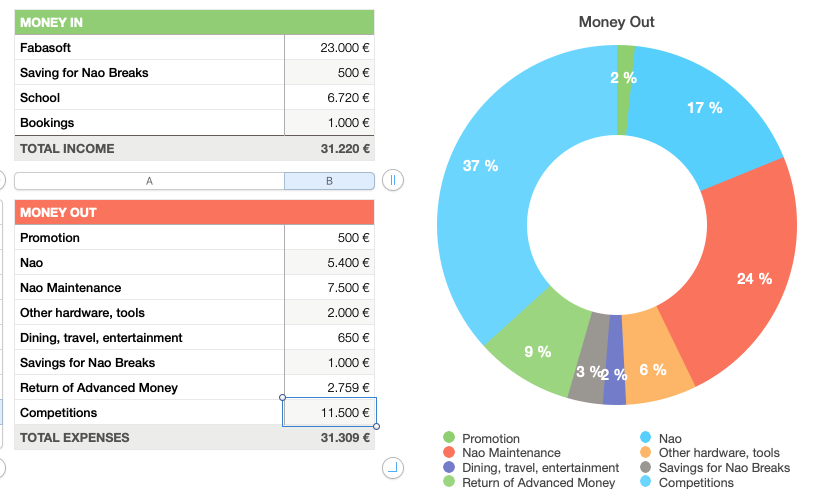
\includegraphics[scale=0.5]{img/budget.png}
\end{center}
\caption{Budget 2019/20}
\label{fig:budget}
\end{figure}

\subsection{Inventory}
Currently we have a total number of eight Naos available in our team. Compared to the last period of report we had to remove three old robots since they ran out of maintenance at SoftBank Robotics. Since we bought four new Naos and we may borrow two more Naos from Fabasoft we are able to play soccer training games already in a full competition setup. Two of the newly bought Naos are basically a purchase of Fabasoft which are loans to our initiative.Table~\ref{tab:naos} lists all available Naos.

\begin{table}
\begin{center}
\begin{tabular}{|p{.3\linewidth}|p{.1\linewidth}|p{.2\linewidth}|}
\hline
\cellcolor{gray!100}\textcolor{white}{Name} & \cellcolor{gray!100}\textcolor{white}{Model} & \cellcolor{gray!100}\textcolor{white}{Year of Purchase} \\ \hline
Ada & V6 & 2020 \\ \hline
Alan & V6 & 2020 \\ \hline
Margaret & V6 & 2019 (Fabasoft) \\ \hline
Linus & V6 & 2019 (Fabasoft) \\ \hline
Donald & V6 & 2018 \\ \hline
Grace & V6 & 2018 \\ \hline
Tom & V5 & 2016 \\ \hline
Anastasia & V5 & 2016 \\ \hline
\end{tabular}
\end{center}
\caption{Currently available Naos}
\label{tab:naos}
\end{table}

\section{Planned Activities for 2020/21}

\begin{itemize}
	\item {\em Public Events:}  Despite COVID-19 and its consequences we still plan to have at least 10 appearances with our Naos.
	
	\item {\em New Nao:} As already mentioned in section~\ref{sec:budget} another V6 will come to our team.
		
	\item {\em RoboCup German Open:} We are eager to finally prove our software at the Standard Platform League at the German Open 2020 in Magdeburg.
\end{itemize}

\section{Acknowledgements}
This project would not be possible without the kind support of several persons and organizations. We would like to express our gratitude to:

\begin{itemize}
	\item \emph{Absolventenverein der HTL Leonding (AbsLeo):} The AbsLeo accompanies this project since 2009. It budgeted the initial hardware which allowed us to get first experience with the Naos, renewed our hardware in Fall 2016, and contributed to the new Naos bought in Fall 2018. Although it was clear that the whole journey will be a long one we could rely on their constant support. This enabled us to continue our ambitions towards participating the RoboCup World Championships.
	
	\item \emph{Management of the HTL Leonding:} Every project needs the great support from its embedding organization. All the smaller and larger organizational issues we are facing can be solved by means of the friendly support of our school. This is enabled by our head master and the two heads of departments. We are very happy to know that we can rely on them.
	
	\item \emph{Thomas Himmelbauer:} Despite his tough schedule as our school's IT manager he is a great technical supporter of our project. Especially if it comes to support our team in the small but important technical questions, from providing power distributions to software tools, he is always a great help.
\end{itemize}

\end{document}  